\section{Observation and Calculations}
Least Count of Calibrated Drum, $\Delta \lambda$ = $1$ nm

\subsection*{Calibration of the spectrometer}

\begin{table}[H]
    \centering
    \begin{tabular}{|c|c|}
    \hline
    $\lambda_{given}$ (nm) & $\lambda_{obs}$ (nm) \\ \hline
    407 & 407 \\ \hline
    435 & 435 \\ \hline
    489 & 489 \\ \hline
    494 & 493 \\ \hline
    546 & 546 \\ \hline
    579 & 579 \\ \hline
    596 & 596 \\ \hline
    615 & 618 \\ \hline
    620 & 624 \\ \hline
    \end{tabular}%
    \caption{Calibration using Hg lamp}
    \label{tab:calib}
\end{table}

\begin{figure}[H]
    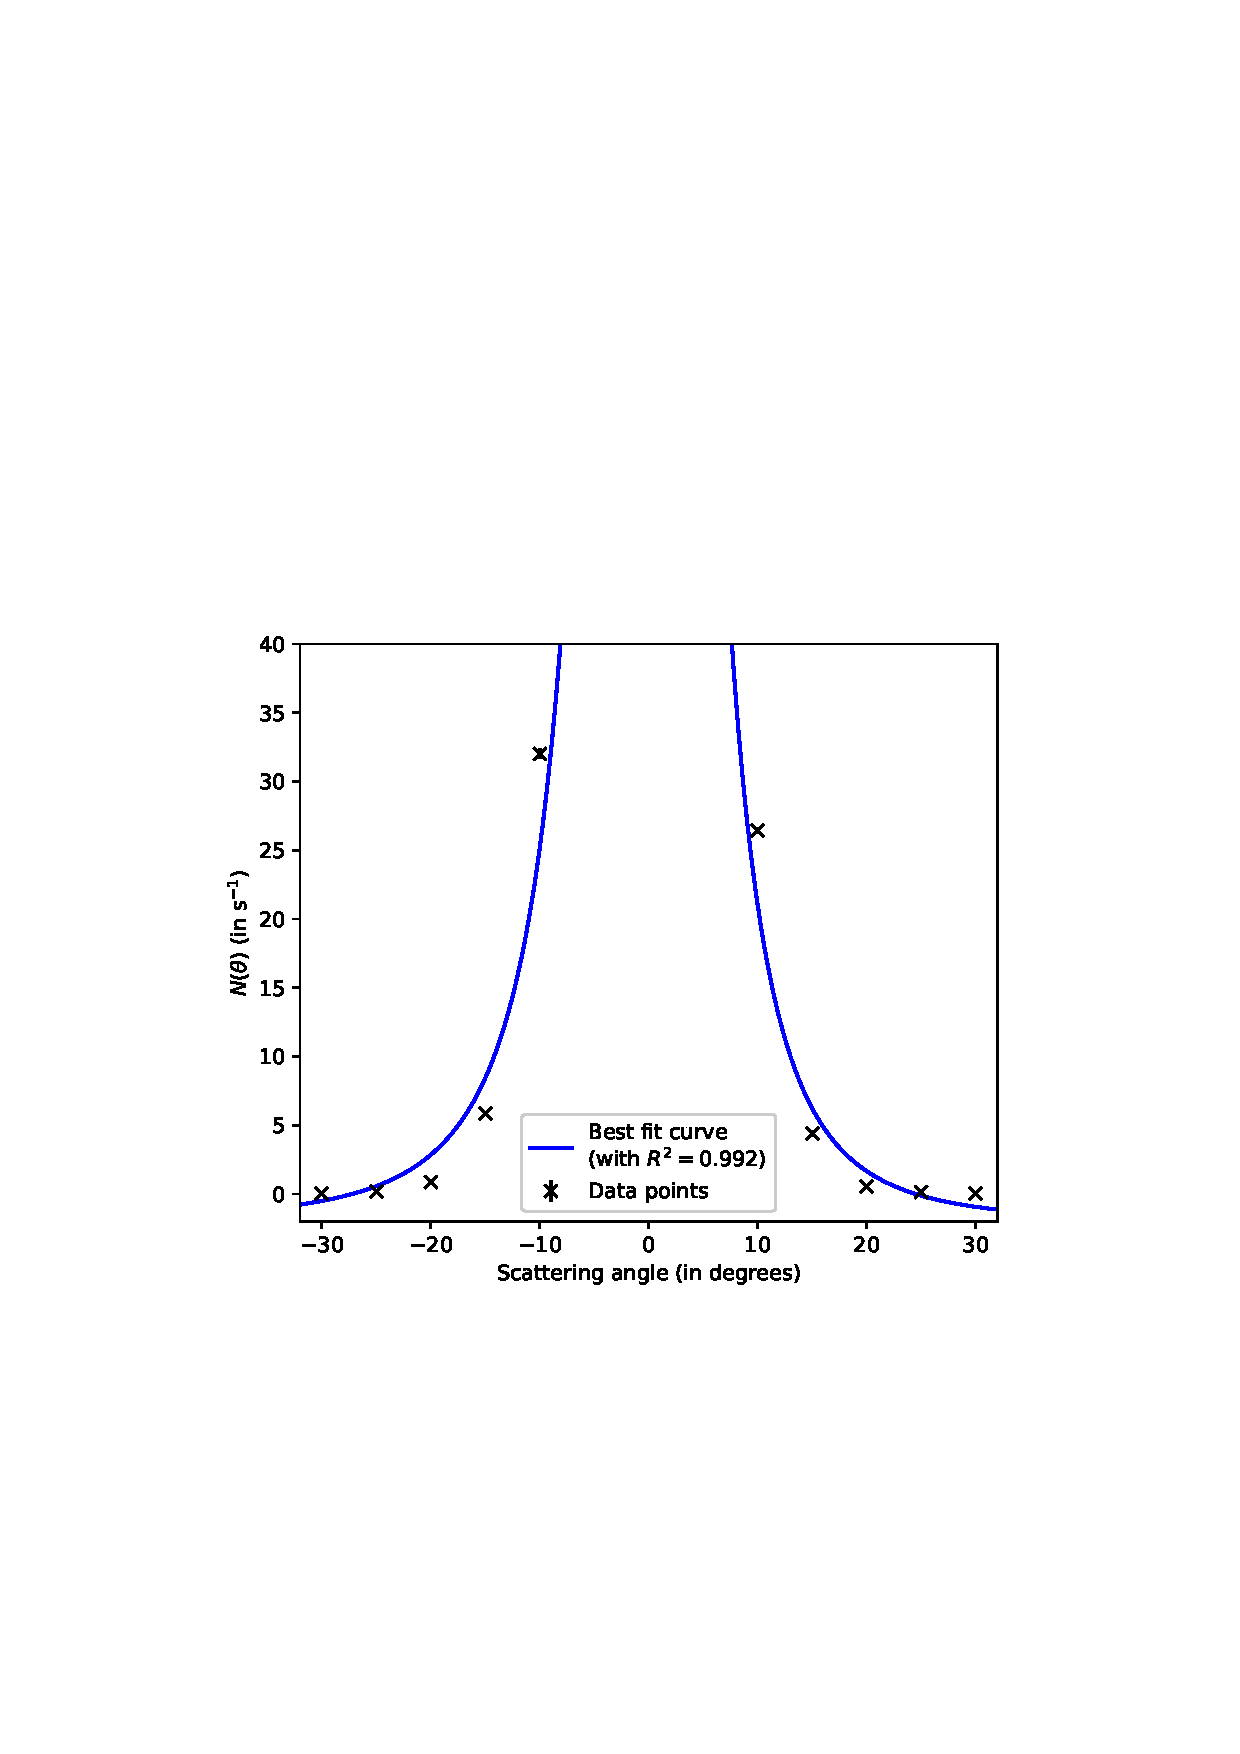
\includegraphics[width=\columnwidth]{images/plt.png}
    \caption{$\lambda_{given}$ vs $\lambda_{obs}$ plot for Hg Spectrum}
    \label{fig:t1}
\end{figure}

From Fig. \ref{fig:t1}, we find the equation for $\lambda_{corr}=0.9806\,\lambda_{obs}+9.42$

\subsection*{Emission Spectra of Metals}

\begin{itemize}
    \item \textbf{For Copper:}
    \begin{table}[H]
        \centering
        \begin{tabular}{|c|c|c|c|}
            \hline
            Color                   & $\lambda_{observed}$   (nm) & $\lambda_{corr}$   (nm) & $\lambda_{lit}$   (nm) \\ \hline
            \multirow{2}{*}{Yellow} & 579                         & 577                     & 581.5                  \\ \cline{2-4} 
                                    & 570                         & 568                     & 574.6                  \\ \hline
            \multirow{3}{*}{Green}  & 521                         & 520                     & 524.5                  \\ \cline{2-4} 
                                    & 514                         & 513                     & 515                    \\ \cline{2-4} 
                                    & 509                         & 509                     & 511                    \\ \hline
            \multirow{2}{*}{Blue}   & 469                         & 469                     & 465.4                  \\ \cline{2-4} 
                                    & 464                         & 464                     & 425.6                  \\ \hline
            \multirow{2}{*}{Violet} & 447                         & 448                     & 405                    \\ \cline{2-4} 
                                    & 427                         & 428                     & 400.3                  \\ \hline
        \end{tabular}
        \caption{Emission Spectrum for Copper}
        \label{tab:copper}
    \end{table}
    
    \item \textbf{For Brass:}
    \begin{table}[H]
        \centering
        \begin{tabular}{|c|c|c|c|}
            \hline
            Color                   & $\lambda_{observed}$   (nm) & $\lambda_{corr}$   (nm) & $\lambda_{lit}$   (nm) \\ \hline
            Red                     & 640                         & 637                     & 645.5                  \\ \hline
            \multirow{2}{*}{Yellow} & 579                         & 577                     & 581.9                  \\ \cline{2-4} 
                                    & 571                         & 569                     & 575.6                  \\ \hline
            \multirow{3}{*}{Green}  & 521                         & 520                     & 514.5                  \\ \cline{2-4} 
                                    & 514                         & 513                     & 515.5                  \\ \cline{2-4} 
                                    & 509                         & 509                     & 523.0                  \\ \hline
            \multirow{2}{*}{Blue}   & 479                         & 479                     & 471.9                  \\ \cline{2-4} 
                                    & 471                         & 471                     & 471.0                  \\ \hline
            \multirow{2}{*}{Violet} & 452                         & 453                     & 426.8                  \\ \cline{2-4} 
                                    & 450                         & 451                     & 403.0                  \\ \hline
        \end{tabular}
        \caption{Emission Spectrum for Brass}
        \label{tab:brass}
        \end{table}
\end{itemize}

\subsection*{Absorption Spectra of Iodine Vapour}

\begin{table}[H]
    \centering
    \begin{tabular}{|c|c|c|c|c|}
        \hline
        $\lambda_\text{obs}$& $\lambda_\text{corr}$ & Wave number & Difference in Wave number\\
        (nm) & (nm) & $\bar{\nu_e}\;(cm^{-1})$ & $\Delta\bar{\nu_e}\;(cm^{-1})$ \\ \hline
        568                         & 566                     & 17655                                  &                                              \\ \hline
        571                         & 569                     & 17564                                  & 91                                           \\ \hline
        575                         & 573                     & 17444                                  & 120                                          \\ \hline
        577                         & 575                     & 17384                                  & 59                                           \\ \hline
        580                         & 578                     & 17296                                  & 88                                           \\ \hline
        585                         & 583                     & 17151                                  & 145                                          \\ \hline
        589                         & 587                     & 17036                                  & 115                                          \\ \hline
        592                         & 590                     & 16951                                  & 85                                           \\ \hline
        596                         & 594                     & 16839                                  & 112                                          \\ \hline
        602                         & 600                     & 16674                                  & 165                                          \\ \hline
        607                         & 605                     & 16539                                  & 135                                          \\ \hline
        610                         & 608                     & 16459                                  & 80                                           \\ \hline
        615                         & 612                     & 16327                                  & 132                                          \\ \hline
        618                         & 615                     & 16249                                  & 78                                           \\ \hline
        622                         & 619                     & 16146                                  & 103                                          \\ \hline
        626                         & 623                     & 16044                                  & 102                                          \\ \hline
        630                         & 627                     & 15944                                  & 100                                          \\ \hline
        635                         & 632                     & 15820                                  & 124                                          \\ \hline
        639                         & 636                     & 15723                                  & 98                                           \\ \hline
    \end{tabular}
    \caption{Absorption Spectrum for Iodine}
    \label{tab:iodine}
    \end{table}

\subsubsection{Calculating bond Dissociation Energy}
    Bond Dissociation Energy, 
    
    \begin{align*}
        D_0&=\;E(\nu'=\nu_{max})-E(\nu'=0)\\
        E(\nu'=\nu_{max})&=hc\nu_{max}\\
        \therefore\;E(\nu'=\nu_{max})&=\frac{17655}{8068}\;eV\\
        E(\nu_{max})&=2.19\;eV
    \end{align*}

    Similarly for lowest energy state

    \begin{align*}
    E(\nu'=0)=hc\nu_{min}&=\frac{15723}{8068}\;eV
    E(\nu_{min})&=1.95\;eV
    \end{align*}

    Therefore $D_0 = 2.19 - 1.95 = 0.24$ eV/molecule

    \subsubsection{Calculation of Force Constant}
    \noindent Force Constant is given by: $f=4\pi^2 \mu\;(c\Delta\bar{\nu_{e^{avg}}})^2$\\\\
    From table \ref{tab:iodine} $\;\Delta\bar{\nu_{e^{avg}}} = 107\;cm^{-1}$\\\\
    Reduced mass $\mu= 1.05\; \times\; 10^{-25}\; kg $\\
    \[\therefore\;f=40.30\;N m^{-1}\]

    \section{Error Analysis}

    \subsection{Bond Dissociation Energy}
        $$\frac{\delta D_0}{D_0} = \frac{\delta E(\nu'=\nu_{max})}{E(\nu'=\nu_{max})} + \frac{\delta E(\nu'=0)}{E(\nu'=0)}$$ 
        $$= hc\left(\frac{\delta \nu_{min}}{\nu_{min}} + \frac{\delta \nu_{max}}{\nu_{max}}\right)$$
        $$\text{now, }\delta \nu (\lambda)= -\frac{\delta\lambda}{\lambda^2}$$
        $$\therefore\; \frac{\delta D_0}{D_0} = -hc\;\delta\lambda\left(\frac{1}{\lambda_{min}^2} + \frac{1}{\lambda_{max}^2}\right) = -8.12\times10^{-3}eV$$
        $$\delta D_0 = -1.94\times10^{-3}\;eV/molecule$$

    \subsection{Force Constant}
        $$\delta f = \frac{2f}{\Delta\bar{\nu_{e^{avg}}}} \; \delta(\Delta\bar{\nu_{e^{avg}}}) = 2\times 40.30 \times \frac{25.69}{107} Nm^{-1}$$
        $$\therefore \delta f = 19.35\;N m^{-1}$$